\documentclass[12pt, onecolumn]{IEEEtran}
\usepackage{graphics,  color,  amsmath, amsfonts, amssymb, balance,algorithm,algorithmic,array ,comment}
\usepackage{graphicx}
%\usepackage{bbding}
%\usepackage{multirow}
\usepackage{caption}
\usepackage{algorithm}
\usepackage{algorithmic}
\usepackage{amsmath, amssymb}
\usepackage{mathrsfs}
\usepackage{bm}%Greek letters in boldface
\vfuzz2pt % Don't report over-full v-boxes if over-edge is small draftcls
\hfuzz2pt % Don't report over-full h-boxes if over-edge is small
% THEOREMS -------------------------------------------------------
\newtheorem{thm}{Theorem}%[section] ,draftcls
\newtheorem{cor}{Corollary}
\usepackage{amsthm}
\newtheorem{lem}{Lemma}
\newtheorem{prop}{Proposition}
\newtheorem{defn}{Definition}
\newtheorem{rem}{Remark}
\newtheorem{example}{Example}
\newtheorem{theorem}{Theorem}
\renewcommand{\algorithmicrequire}{ \textbf{Initialization:}}
\renewcommand{\algorithmicensure}{ \textbf{Return:}}

\author{Jianxin Dai\\
}
\title{Discuss Report }
\begin{document}
\maketitle


\section{Introduction}

In the paper \cite{geraci2017operating}, authors proposed to operate massive Multiple Input Multiple Output (MIMO) cellular Base Stations (BSs) in unlicensed bands (mMIMO-U). They design a procedures required at a cellular BS to guarantee coexistence with nearby WiFi stations in the same piece of unlicensed band via interference alignment technology.  Fig.~\ref{FIG:mMIMO} show the flow of mMIMO-U  proposed.
\begin{figure}[H]
    \centering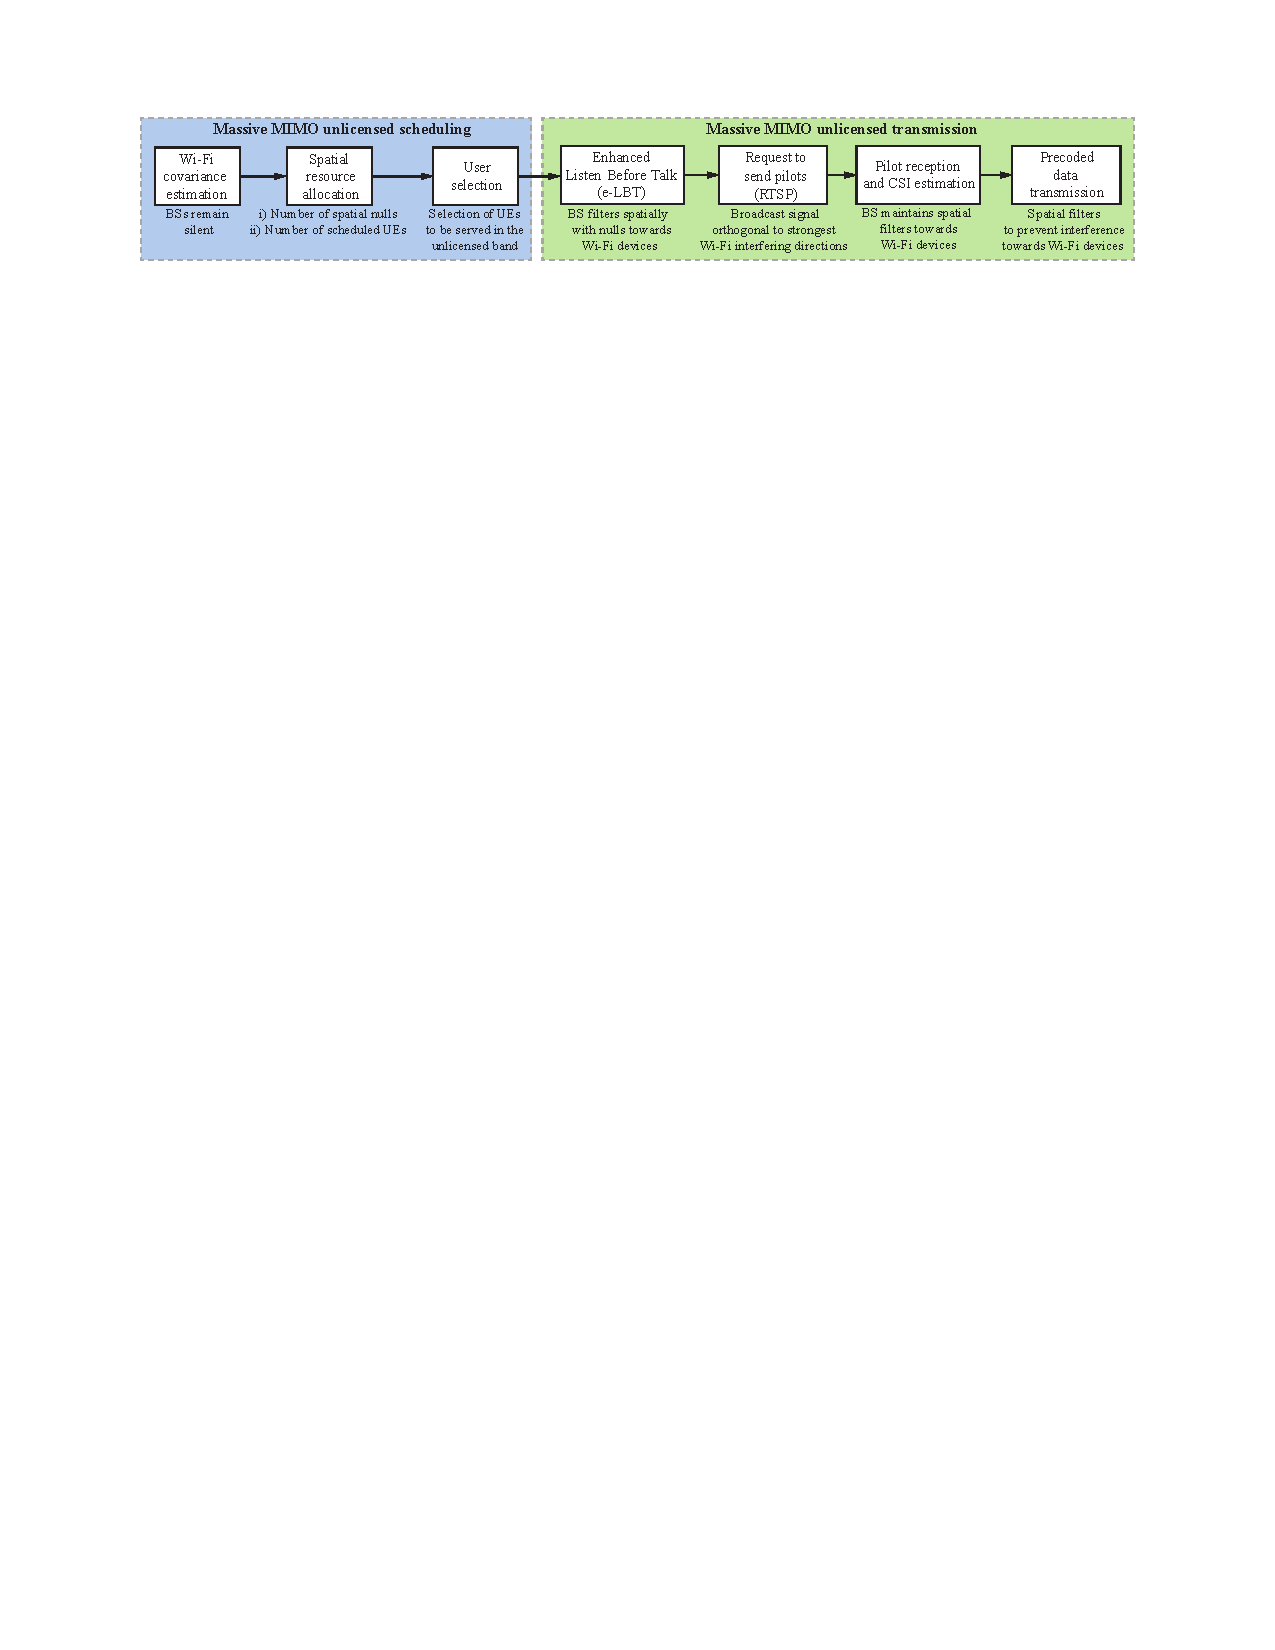
\includegraphics[width=1\columnwidth]{mMIMO.pdf}
    \caption{ Flow chart of the proposed mMIMO-U}\label{FIG:mMIMO}
\end{figure}
\begin{description}
  \item[Step1:] %authors discuss the operations requires for a massive MIMO celluar BS to:
                    \begin{enumerate}
                      \item acquire channel state information from the neighboring WiFi devices.
                      \item allocate spatial resources for WiFi interference suppression and user equipment (UE) multiplexing.
                      \item select a suitable set of UEs to be served in the unlicensed band.
                    \end{enumerate}
  \item[Step2:] %authors devise a transmission operations of a massive MIMO-U system, including:
                    \begin{enumerate}
                        \item an enhanced LBT phase.
                        \item procedures for UE pilot request and channel estimation.
                        \item precoder calculation.
                    \end{enumerate}
\end{description}


\section{System Model}

  WE consider the downlink of a cellular network where  massive MIMO cellular BSs are deployed to operate in the unlicensed band in a synchronous manner, and communicate with their respective sets of connected cellular UEs, while WiFi devices also operate in the same unlicensed band.  Each BSs equipped with  a larger number of antennas $N$, and  simultaneously serves K UEs. Each BS transmit with power $P_{b}$. On the WiFi side, $L$ is denoted by the set of WiFi devices. We assume that all WiFi device transmit with power $P_{w}$.  It worth nothing that both UEs and WiFi devices are equipped with one antenna.  Without loss of generality, we also assume the same symbol duration for cellular and WiFi transmission. Thus the   signal $y_{(i,k)}\in{}\mathbb{C}$ received by  UE $k$ in cell $i$   can  be expressed as
 \begin{equation}\label{EQU:ChannelModel}
    \begin{aligned}
        y_{(i,k)}[m] = & \sqrt{P_{b}}h_{[i,(i,k)]}w_{(i,k)}s_{(i,k)}[m] + \sqrt{P_{b}}\sum_{k'\in{}K_{i}\backslash{}k}h_{[i,(i,k)]}w_{(i,k')}s_{(i,k')}[m] +  \\ & \sqrt{P_{b}}\sum_{i'\in{}J\backslash{}k}h_{[i',(i,k)]}w_{(i',k)}s_{(i',k)}[m] +    \sqrt{P_{w}}\sum_{l\in{}L}g_{[l,(i,k)]}s_{(l)}[m]  +  \eta[m]
    \end{aligned}
\end{equation}
where $h_{[i,(j,k)]} \in{}\mathbb{C}^{1\times{}N}$ is denoted as the channel vector between BS $i$ and UE $k$ in cell$j$.  $g_{[l,(j,k)]} \in{}\mathbb{C}$ is denoted as the channel coefficient  between WiFi device $l$ and UE  $k$ in cell $j$. $w_{(i,k)}\in{}\mathbb{C}^{N\times{}1}$ is the precoding vector from BS $i$ to UE $k$, $s_{(i,k)}\in{}\mathbb{C}$ and $s_{(l)}\in{}\mathbb{C}$ is the unit-variance signal transmitted by BS $i$ and WiFi $l$, respectively.  $\eta[m]\sim \mathcal{CN}(0,1)$ is the thermal noise.
\subsection{WiFi Channel Estimation}
In this phase, all the BSs remain silent, and thus each BSs $i$  receives the signal from neighboring  WiFi devices. We can obtain the interference  estimation by
\begin{equation}
    \begin{aligned}
        & z_{i}[m] = \sum_{l\in{}L} \sqrt{P_{w}}g_{i,l}s_{l} + \eta_{i}[m] \\
        & Z_{i} = \frac{1}{M_{c}}\sum_{m=1}^{M_{c}} z_{i}[m]z_{i}^{\dag}[m],
    \end{aligned}
\end{equation}
which consists of all transmission from active WiFi devices and noise term $\eta$ is AGWN. The $M_{c}$ is the length symbol intervals BS keep silent. $g_{i,l}\in{}\mathbb{C}^{N\times{}1}$ is denoted as the channel vector between  BS $i$ and WiFi $l$. $ Z_{i}\in\mathbb{C}^{N\times{}N}$ is denoted by the estimation covariance of average $Z_{i}[m]$. Given the estimation $Z_{i}$, BS $i$ applies a spectral decomposition, obtaining
\begin{equation}
    \begin{aligned}
        & Z_{i} = U_{i}\Lambda_{i}U^{\dag}_{i},
    \end{aligned}
\end{equation}
where $\Lambda = diag(\lambda_{i,1},,,\lambda_{i,N})$, such that $\lambda_{i,1}>\lambda_{i,1},,,>\lambda_{i,N})$.  In order to  allocate Degree of Freedom (DoF), let define the matrix
\begin{equation}
    \begin{aligned}
        \Sigma_{i} = [u_{i,1},,,u_{i,D_{i}}],
    \end{aligned}
\end{equation}
whose columns contain the $D_{i}$ dominant eigenvectors of $Z_{i}$. For a sufficiently large $D_{i}$, $range\{\Sigma_{i}\}$ represents the channel subspace on which BSs $i$ receives most of the WiFi transmitted power. Therefore, the power transmitted by BS $i$  on $range\{\Sigma_{i}\}$ represents the major source of the interference for one or more WiFi devices.

\section{My Question}
It is well known that WiFi applied Carrier Sense Multiple Access with Collision Avoidance (CSMA/CA) protocol which channel will be occupied by only one  device in one time slot.  Therefore it is ineffective that this method  estimate channel state information from neighboring WiFi device. It is obvious that this method will estimate  major WiFi devices which active with high frequency. Let us consider this case, there is a WiFi  device  active with low frequency. On the hand, this estimation method will not guarantee this WiFi signal space. On the other hand, the estimation from major WiFi devices will be inaccurate due to this  WiFi device.  


It is better(maybe) method that we can compute estimation by selecting major WiFi devices. 


\section{My plan}
Some  simulations may be need for verifying my idea.  

%\bibliographystyle{ieeetr}
\bibliographystyle{hieeetran}
\bibliography{MyCite}
\end{document}
